
\subsection{Classifying Arcs, Ovals and Hyperovals}


A set of points in the Desarguesian 
projective plane $\PG(2,q)$ 
is called an {\em arc} 
if no three points of the set are collinear (i.e., lie on a line). 
Thus, an arc is a set of points that intersects any line in at most 2 points. 
It is known that that an arc has 
size at most $q+2.$ If $q$ is odd, this bound can be improved to $q+1.$
Arcs of size $q+1$ are called {\em ovals} and arcs of size $q+2$ are called {\em hyperovals.} 
Examples for ovals are the {\em conics}, i.e., the zero-sets of nondegenerate homogeneous quadratic polynomials in three 
variables.
By a theorem of Segre, ovals in $\PG(2,q)$ with $q$ odd are conics.  
For $q$ even, ovals are known that are 
not conics. 
Hyperovals arise from ovals using the following procedure. 
Consider the set of tangent lines to the oval 
(a tangent line is a line intersecting the oval in exactly one point; there is exactly one tangent line 
at each point of the oval). 
It is well-known that the set of $q+1$ tangent lines to an oval 
intersect in a unique point, called the {\em nucleus} of the oval. 
The oval together with the nucleus gives rise to a hyperoval.
If the oval is a conic, the resulting hyperoval is called a {\em hyperconic.}
However, not every hyperoval must be a hyperconic. 

\bigskip

A full classification of ovals and hyperovals 
seems to be beyond reach at the moment.
For this reason, there is great interest in 
using the computer to classify ovals and hyperovals in 
small order projective planes.
The computer can give us examples of hyperovals that any classification would 
have to include.
Hyperovals have been classified for $q \le 32.$ 
We can use \verb'orbiter' to reproduce these classifications 
on a laptop machine. 
However, the case of hyperovals in $\PG(2,64)$ seems 
to be beyond reach. 

\bigskip

 
The program that we will use is called \verb'hyperoval.out' and resides in 
\begin{quote}
\verb'ORBITER/SRC/APPS/HYPEROVAL'
\end{quote}
There is a \verb'makefile' in 
\begin{quote}
\verb'ORBITER/DATA/HYPEROVAL'
\end{quote}
that we can use. 
The main body of the program is the class \verb'arc_generator' in 
\begin{quote}
\verb'ORBITER/SRC/APPS/HYPEROVAL/arc_generator.C'
\end{quote}
The class \verb'arc_generator' maintains the projective plane 
$\PG(2,q)$ together with its group $\PGGL(3,q).$
The incidence structure of the plane is encoded in an object 
\begin{quote}
\verb'projective_space *P2;'
\end{quote}
that is initialized using the commands
\begin{quote}
\verb'P2 = new projective_space;'\\
\verb'P2->init(2, q, FALSE /* f_init_group */, '\\
\verb'    f_semilinear, NULL /*const BYTE *override_poly*/, FALSE /* f_basis */, '\\
\verb'    0 /*verbose_level - 2*/);'\\
\end{quote}
This command sets up a $2$-dimensional projective space defined over the field $\bbF_q.$
The group is maintained in an \verb'action' object named 
\verb'A', initialized via
\begin{quote}
\verb'A->init_matrix_group(TRUE /* f_projective */, 3, q, '\\
\verb'    "" /*override_poly*/, f_semilinear, f_basis, 0 /*verbose_level*/);'\\
\end{quote}
This sets up a $3$-dimensional matrix group acting on projective space. 
The flag \verb'f_semilinear' has previously been set to \verb'TRUE' if $q$ is not a prime. This flag determines whether we create the semilinear group.
The flag \verb'f_basis' is \verb'TRUE' and implied that a stabilizer 
chain for the group is constructed.
Two objects are implicitly set up. The first is an object of type \verb'matrix_group', 
the second is an object of type \verb'finite_field'.
The objects are initialized using the following commands
\begin{quote}
\verb'matrix_group *M;'\\
\verb'finite_field *F;'\\
\verb'M = A->G.matrix_grp;'\\
\verb'F = M->GFq;'\\
\end{quote}
Since we will need the action on the set of lines also, we have 
a separate \verb'action' object \verb'A_on_lines'. This is initialized 
by first setting up an object of type 
\verb'action_on_grassmannian'. The whole sequence of commands is
\begin{quote}
\verb'A_on_lines = new action;'\\
\verb'AG = new action_on_grassmannian;'\\
\verb'AG->init(*A, 3 /*n*/, 2 /*k*/, q, F, verbose_level - 2);'\\
\verb'A_on_lines->induced_action_on_grassmannian(A, AG,'\\
\verb'    FALSE /*f_induce_action*/, NULL /*sims *old_G */, '\\
\verb'    MINIMUM(verbose_level - 2, 2));'\\
\end{quote}
Observe that the object \verb'finite_field *F' is needed to set up the 
\verb'action_on_grassmannian' object \verb'AG', which in turn is needed to set up 
the \verb'action' object \verb'A_on_lines'.

\bigskip






Inside \verb'ORBITER/DATA/HYPEROVAL', we could issue any of the commands 
\begin{quote}
\verb'make 8' \\
\verb'make 16'\\
\end{quote}
to classify the hyperovals in $\PG(2,8)$ and $\PG(2,16)$, respectively.
This algorithm classifies the orbits of $\PGGL(2,q)$ 
on arcs in $\PG(2,q).$
The results will be in the files
\begin{quote}
\verb'ORBITER/DATA/HYPEROVAL/CLASSIFY_8/arc_8_lvl_10'\\
\verb'ORBITER/DATA/HYPEROVAL/CLASSIFY_16/arc_16_lvl_18'\\
\end{quote}
In $\PG(2,8),$ the only hyperoval is the hyperconic.
In $\PG(2,16),$ there are two hyperovals. 
One is the hyperconic, and the other is the Lunelli-Sce hyperoval. 
They both can be found in the file \verb'CLASSIFY_16/arc_16_lvl_18' (which -- 
as pointed out before -- is only semi-readable for humans). 
The search tree for the hyperovals in $\PG(2,16)$ has 4214 nodes and looks like this:
$$
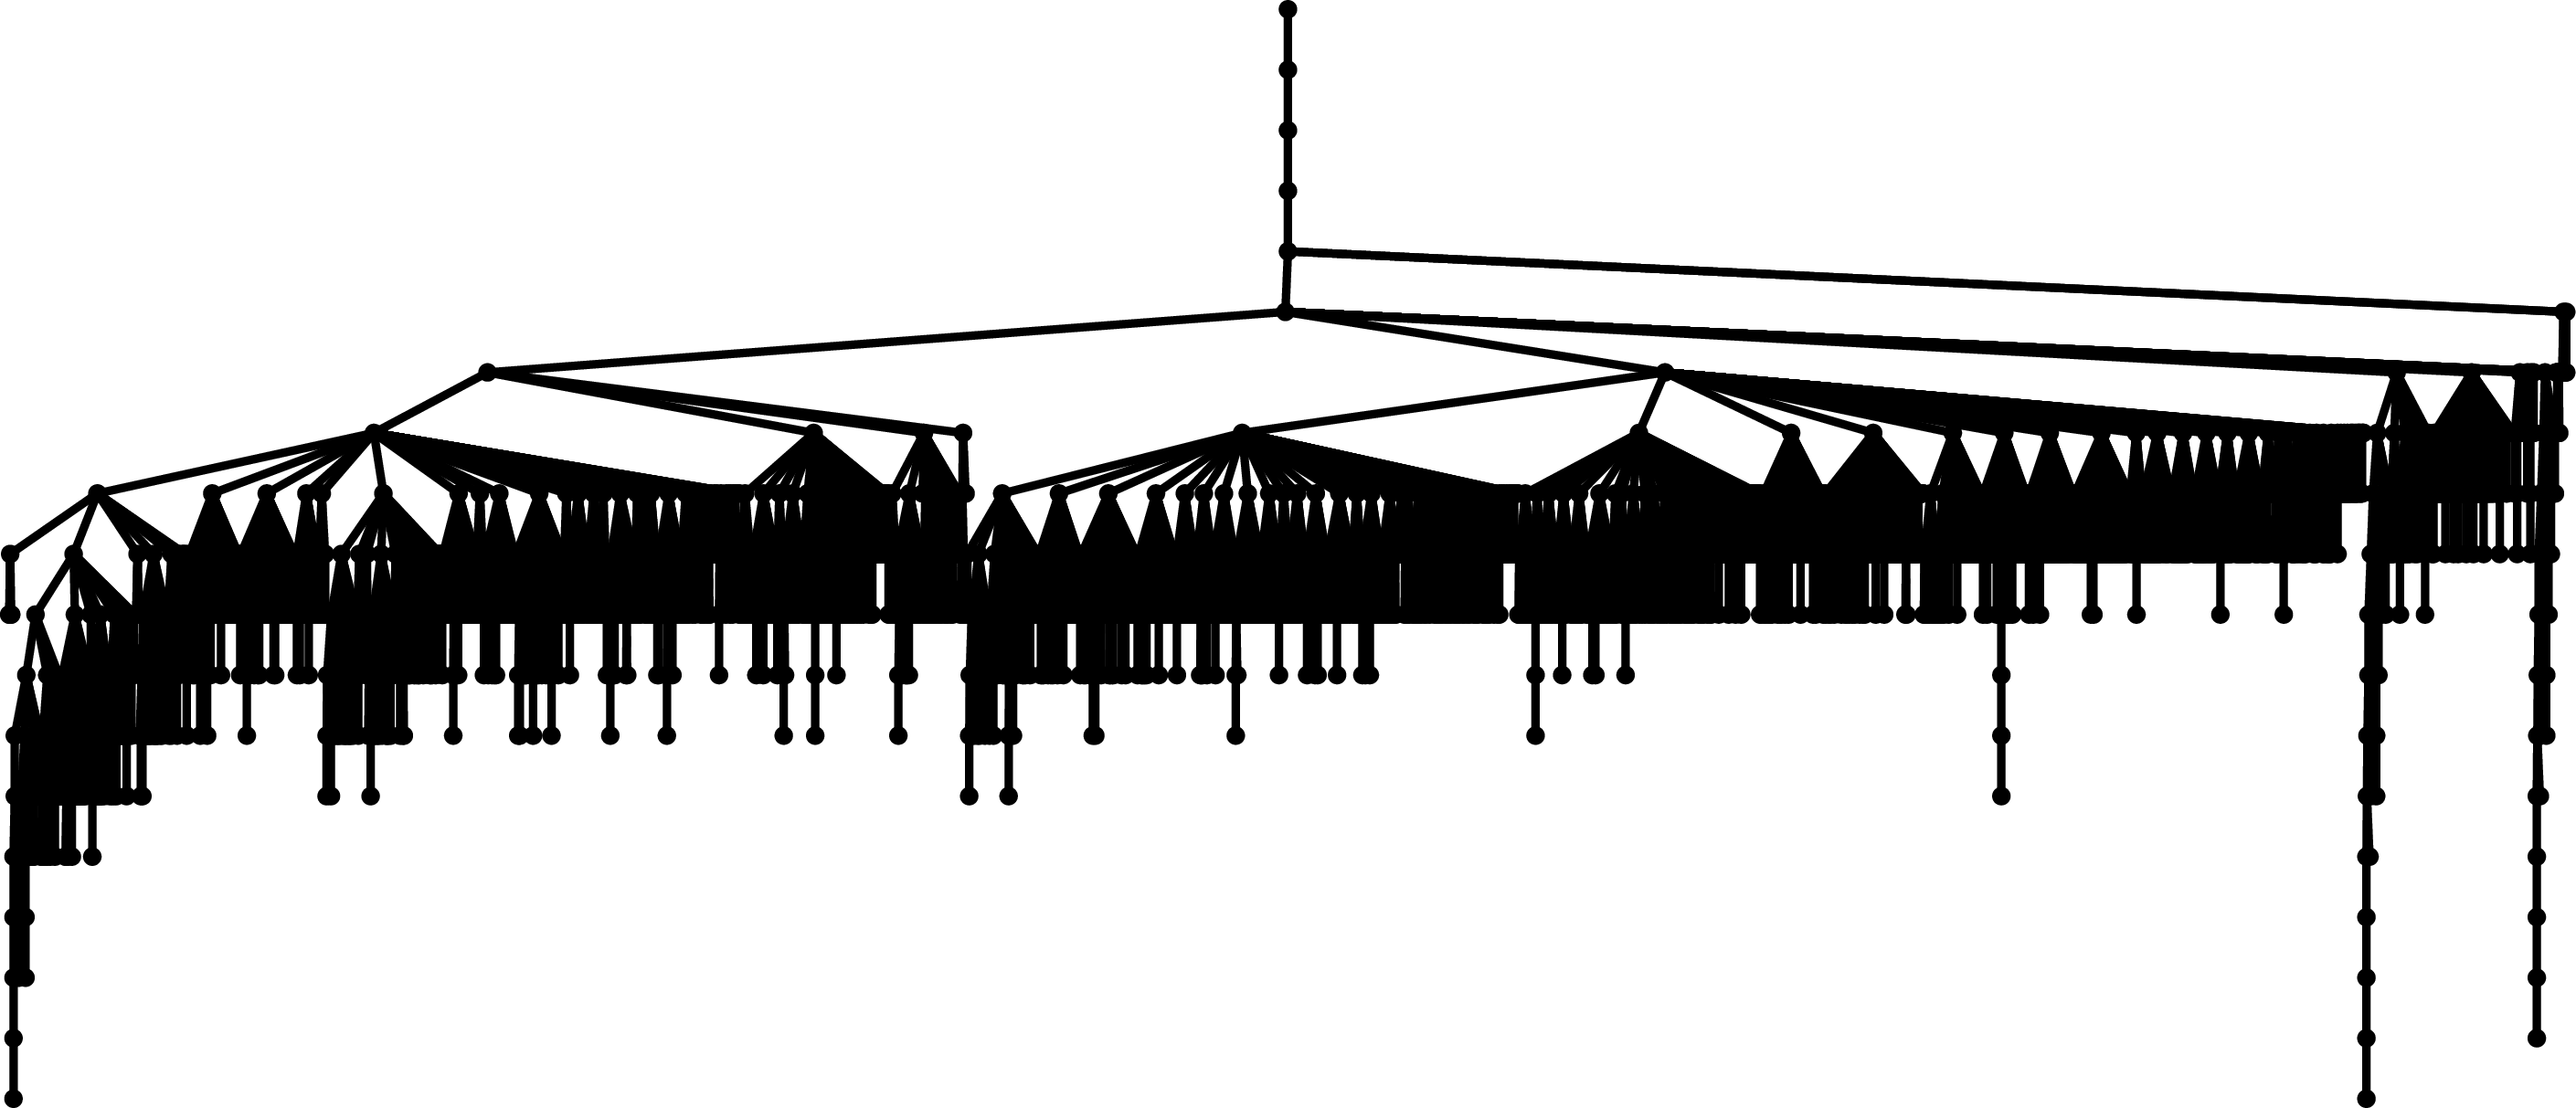
\includegraphics[width=150mm]{GRAPHICS/hyperoval_16_tree}
$$
With this tree, we can already spot the problem with this classification method. 
The tree is quite ``bushy.'' A great number of intermediate nodes run dead quickly, preventing this method from being effective for larger problem sizes.
In order to proceed to larger instances of the 
problem of classifying hyperovals, 
we need to employ a different search method.








